\chapter{System Architecture and API Backbone}
\label{chap:architecture}

\section{Scope of the Architecture Work}

This chapter describes the technical backbone implemented around Kafka, HDFS, and the Flask REST API. In the RAPID platform, the backbone has three responsibilities. First, it provides the ingestion and storage path that keeps the cybersecurity log stream reproducible. Second, it connects the batch and speed computations to a consistent serving model. Third, it exposes the results through a REST interface that can be consumed by the dashboard, integration scripts, and external security tools. The implementation follows a Lambda Architecture because the problem has two distinct requirements: high-throughput historical analytics over a complete log corpus, and low-latency detection over newly arriving events \cite{marz2015bigdata}.

The deployed system is distributed across several team machines connected through a private Tailscale network and a Docker Swarm overlay network. Anass' node hosts Zookeeper, Kafka, the HDFS NameNode/DataNode pair, and the Flask API. Spark jobs run from the Spark profiles, while Cassandra and HBase are hosted on Chawi's node. This separation is important academically and operationally: it demonstrates that the platform is not only a local script pipeline, but a multi-service data architecture with explicit network boundaries, storage responsibilities, and serving interfaces.

\section{Global Architecture}

Figure~\ref{fig:lambda-architecture} presents the high-level flow. The raw dataset is first organized in HDFS as monthly partitions. HDFS is the durable source of truth for replayable cybersecurity events, while Kafka acts as the temporal buffer used by the speed layer. Spark consumes both sides of the architecture: batch jobs scan HDFS to produce historical summaries, and streaming jobs consume Kafka to update real-time Cassandra tables. The Flask API then bridges Cassandra and HBase so that a single endpoint can return both recent state and historical reputation.

\begin{figure}[H]
    \centering
    \resizebox{\textwidth}{!}{\begin{tikzpicture}[
    font=\small,
    box/.style={draw, rounded corners=3pt, align=center, minimum height=1.0cm, text width=3.0cm, fill=white},
    store/.style={draw, cylinder, shape border rotate=90, aspect=0.22, align=center, minimum height=1.15cm, text width=2.8cm, fill=white},
    layer/.style={draw, rounded corners=5pt, dashed, inner xsep=0.35cm, inner ysep=0.28cm},
    arrow/.style={-{Latex[length=2.5mm]}, thick, shorten >=2pt, shorten <=2pt},
    streamline/.style={arrow, rapidOrange},
    batchline/.style={arrow, rapidBlue},
    serveline/.style={arrow, rapidGreen}
]

\node[box, fill=rapidLight] (dataset) at (0,0) {Cybersecurity\\CSV logs};
\node[store, fill=rapidLight] (hdfs) at (3.9,0) {HDFS\\raw partitions};

\node[box, fill=rapidOrange!12] (producer) at (7.4,1.75) {Kafka replay\\producer};
\node[box, fill=rapidOrange!12] (kafka) at (11.0,1.75) {Kafka topic\\\texttt{cybersecurity}\\\texttt{logs}};
\node[box, fill=rapidOrange!12] (streamjob) at (14.6,1.75) {Spark Structured\\Streaming jobs};
\node[store, fill=rapidOrange!12] (cassandra) at (18.2,1.75) {Cassandra\\real-time views};

\node[box, fill=rapidBlue!10] (batchspark) at (8.4,-1.75) {Spark batch\\analytics};
\node[store, fill=rapidBlue!10] (hbase) at (12.4,-1.75) {HBase\\historical views};

\node[box, fill=rapidGreen!12] (api) at (18.2,-1.75) {Flask REST API\\serving bridge};
\node[box, fill=rapidGreen!12] (dashboard) at (22.0,-1.75) {Dashboard and\\client queries};

\draw[arrow] (dataset) -- (hdfs);
\draw[streamline] (hdfs.north) |- (producer.west);
\draw[streamline] (producer) -- (kafka);
\draw[streamline] (kafka) -- (streamjob);
\draw[streamline] (streamjob) -- (cassandra);

\draw[batchline] (hdfs.south) |- (batchspark.west);
\draw[batchline] (batchspark) -- (hbase);

\draw[serveline] (cassandra.south) -- (api.north);
\draw[serveline] (hbase) -- (api);
\draw[serveline] (api) -- (dashboard);

\begin{scope}[on background layer]
    \node[layer, fit=(producer)(kafka)(streamjob)(cassandra), label={[rapidOrange]above:Speed layer}] {};
    \node[layer, fit=(batchspark)(hbase), label={[rapidBlue]below:Batch layer}] {};
    \node[layer, fit=(api)(dashboard), label={[rapidGreen]below:Serving layer}] {};
\end{scope}

\end{tikzpicture}
}
    \caption{RAPID Lambda Architecture: HDFS keeps replayable raw logs, Kafka carries the live stream, Spark computes batch and speed views, and the Flask API unifies Cassandra and HBase outputs.}
    \label{fig:lambda-architecture}
\end{figure}

\section{Infrastructure Motivation}

The infrastructure design was not chosen only for demonstration. A complete RAPID stack contains Kafka, Zookeeper, HDFS, Spark, Cassandra, HBase, Flask, and the dashboard. Running all of these services on one machine creates resource contention in four places: CPU scheduling, memory pressure, disk input/output, and network ports. This is especially visible in a big-data project because Spark can consume large memory while Cassandra and HBase also need stable heap space, and Kafka/HDFS need reliable disk and network throughput. A single laptop can start the stack in a simplified demo, but it cannot represent the behavior of a real analytical platform under sustained ingestion and processing load.

The project therefore uses a distributed deployment where each machine owns a clear role. This makes the system more realistic: ingestion, compute, serving storage, and API access are separated into different nodes, just as a production data platform separates brokers, compute workers, databases, and application gateways. Figure~\ref{fig:single-host-vs-distributed} summarizes the architectural decision.

\begin{figure}[H]
    \centering
    \resizebox{\textwidth}{!}{\begin{tikzpicture}[
    font=\small,
    panel/.style={draw, rounded corners=6pt, fill=rapidLight, minimum width=6.4cm, minimum height=8.6cm},
    title/.style={font=\bfseries, align=center},
    service/.style={draw, rounded corners=4pt, align=center, minimum width=4.9cm, minimum height=0.82cm, fill=white},
    host/.style={draw, rounded corners=4pt, align=center, text width=3.35cm, minimum height=1.25cm, fill=white},
    note/.style={draw, rounded corners=4pt, align=center, text width=5.3cm, minimum height=1.05cm, fill=white},
    arrow/.style={-{Latex[length=2.6mm]}, thick, rapidGreen, shorten >=4pt, shorten <=4pt}
]

\node[panel] (singlePanel) at (0,0) {};
\node[title] at (0,3.55) {Single-host prototype};

\node[service, fill=rapidOrange!12] at (0,2.55) {Kafka and Zookeeper};
\node[service, fill=rapidBlue!10] at (0,1.55) {HDFS NameNode and DataNode};
\node[service, fill=rapidBlue!10] at (0,0.55) {Spark batch and streaming};
\node[service, fill=rapidOrange!12] at (0,-0.45) {Cassandra and HBase};
\node[service, fill=rapidGreen!12] at (0,-1.45) {Flask API and dashboard};
\node[note, draw=rapidRed, fill=rapidRed!8] at (0,-3.05) {All workloads compete for CPU, memory, disk I/O, and ports};

\node[note, draw=rapidGreen, fill=rapidGreen!8, text width=3.7cm] (decision) at (7.0,0) {Scale out by service responsibility};

\node[panel, minimum width=9.5cm] (distPanel) at (14.2,0) {};
\node[title] at (14.2,3.55) {Distributed RAPID deployment};

\node[host, fill=rapidGreen!12] at (11.15,2.20) {Anass\\Kafka, HDFS, Flask API};
\node[host, fill=rapidBlue!10] at (15.05,2.20) {Hamza\\Spark master and worker};
\node[host, fill=rapidBlue!10] at (11.15,0.40) {Khalid\\Spark streaming detectors};
\node[host, fill=rapidOrange!12] at (15.05,0.40) {Chawi\\Cassandra, HBase, dashboard};

\node[note, fill=white, text width=7.2cm] at (13.10,-1.55) {Tailscale connects the machines; Docker Swarm connects the containers};
\node[note, draw=rapidGreen, fill=rapidGreen!8, text width=7.2cm] at (13.10,-3.05) {Ingestion, compute, serving storage, and API access are separated};

\draw[arrow] (singlePanel.east) -- (decision.west);
\draw[arrow] (decision.east) -- (distPanel.west);

\end{tikzpicture}
}
    \caption{From a single overloaded host to a distributed deployment where each machine carries a specialized part of the big-data workload.}
    \label{fig:single-host-vs-distributed}
\end{figure}

\section{Scrum Planning and Sprint Backlog}

The implementation was managed through a Scrum-style GitHub project board. The backlog was organized around the same technical layers used by the architecture: batch processing, speed processing, serving integration, visualization, documentation, and infrastructure. This helped the team avoid treating the system as one large undifferentiated task. Each card had an owner, a sprint, and a concrete deliverable, which made the distributed deployment easier to coordinate.


\begin{table}[H]
    \centering
    \caption{Scrum backlog summary extracted from the project planning board.}
    \label{tab:scrum-backlog-summary}
    \begin{tabularx}{\textwidth}{>{\bfseries}l l X}
        \toprule
        Sprint & Main theme & Representative deliverables \\
        \midrule
        Sprint 1 & Batch layer and base infrastructure & Docker environment, partitioned HDFS layout, dataset loading, Spark batch analytics, Cassandra schema, HBase tables, and initial test scripts \\
        Sprint 2 & Speed layer & Kafka topic validation, cross-node Cassandra access, CSV-to-Kafka replay producer, Spark Structured Streaming writers, brute-force detection, signature detection, abnormal-volume detection, and real-time threat scoring \\
        Sprint 3 & Integration and delivery & Flask API endpoints, adaptive scoring, top-10 and timeline views, dashboard pages, end-to-end demonstration script, and technical report material \\
        Sprint 4 & Bonus improvements & MLlib classification, model evaluation, multi-step attack correlation, GeoIP enrichment, and dashboard map visualization \\
        \bottomrule
    \end{tabularx}
\end{table}

Figure~\ref{fig:scrum-board-sprint1} shows the first project-board view. Sprint 1 focused on making the base data platform work: setting up the Docker environment, loading and partitioning the dataset, creating HDFS and HBase structures, and implementing early Spark batch analytics. This sprint reduced the main technical risk because all later work depended on having a stable dataset and reproducible base services.

\begin{figure}[H]
    \centering
    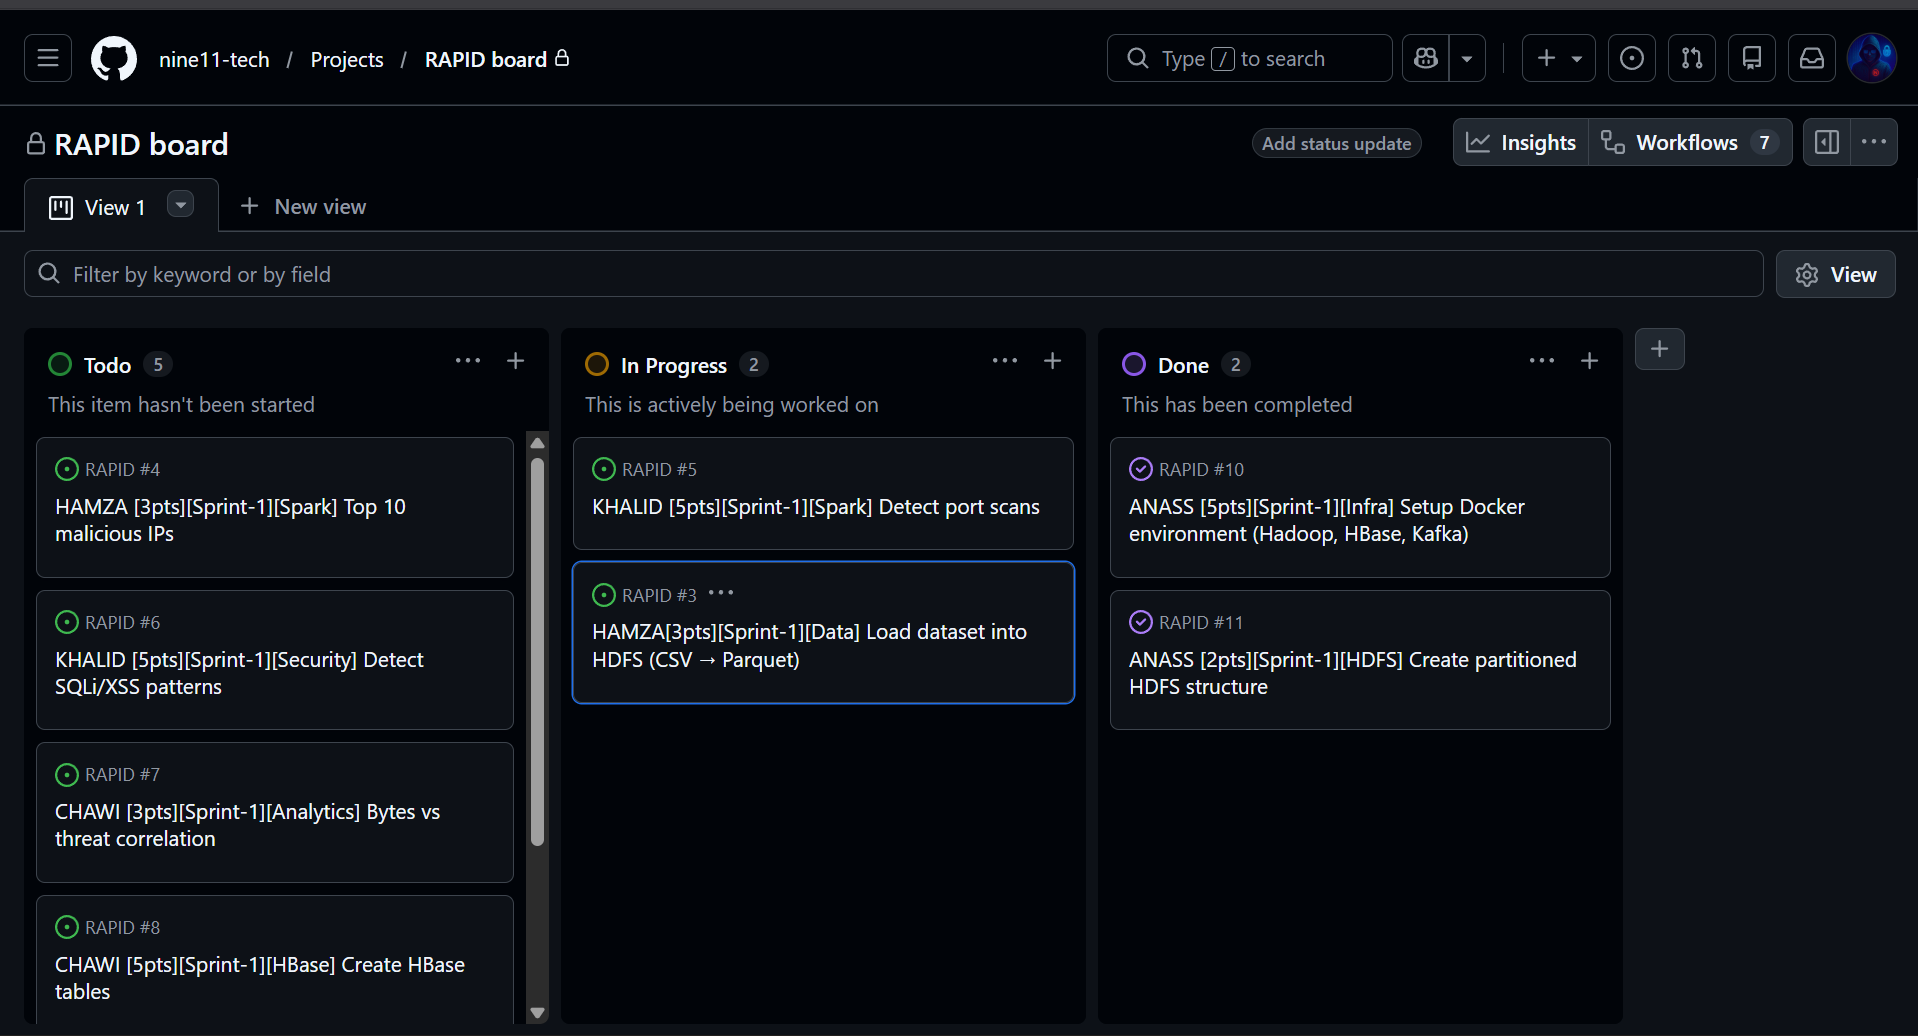
\includegraphics[width=\textwidth]{figures/board1.png}
    \caption{GitHub project board for Sprint 1, focused on the batch layer and base infrastructure.}
    \label{fig:scrum-board-sprint1}
\end{figure}

Figure~\ref{fig:scrum-board-sprint2} shows the second sprint. The board moves the work from offline computation to streaming: Kafka validation, real-time replay from CSV, Spark streaming jobs, Cassandra writes, and detectors for brute-force, signature, and volume-based threats. This sprint is also where cross-machine communication became essential because the streaming container, Kafka broker, and Cassandra service were not all on the same host.

\begin{figure}[H]
    \centering
    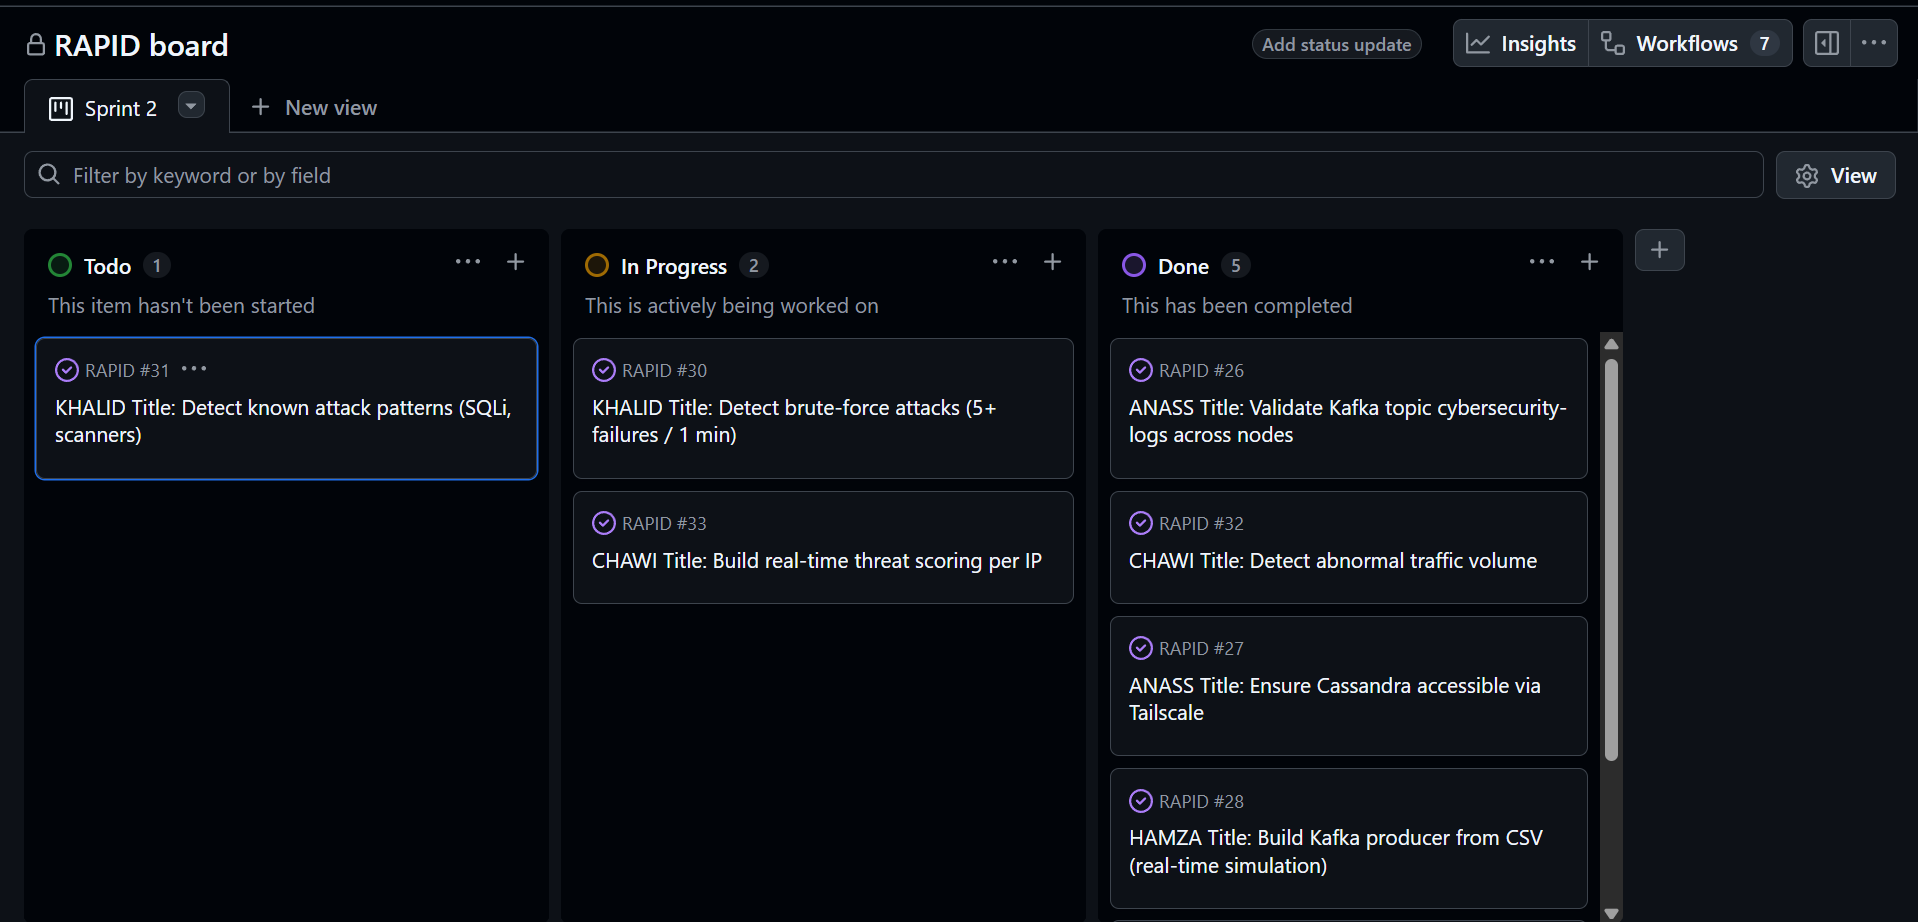
\includegraphics[width=\textwidth]{figures/board2.png}
    \caption{GitHub project board for Sprint 2, focused on Kafka, Spark Streaming, Cassandra writes, and real-time detectors.}
    \label{fig:scrum-board-sprint2}
\end{figure}

Figure~\ref{fig:scrum-board-sprint3} shows the third sprint. The tasks shifted toward integration: API endpoints, adaptive scoring, dashboard pages, an end-to-end demo, and the written technical report. This sprint connected the individual layer outputs into a user-facing security monitoring workflow.

\begin{figure}[H]
    \centering
    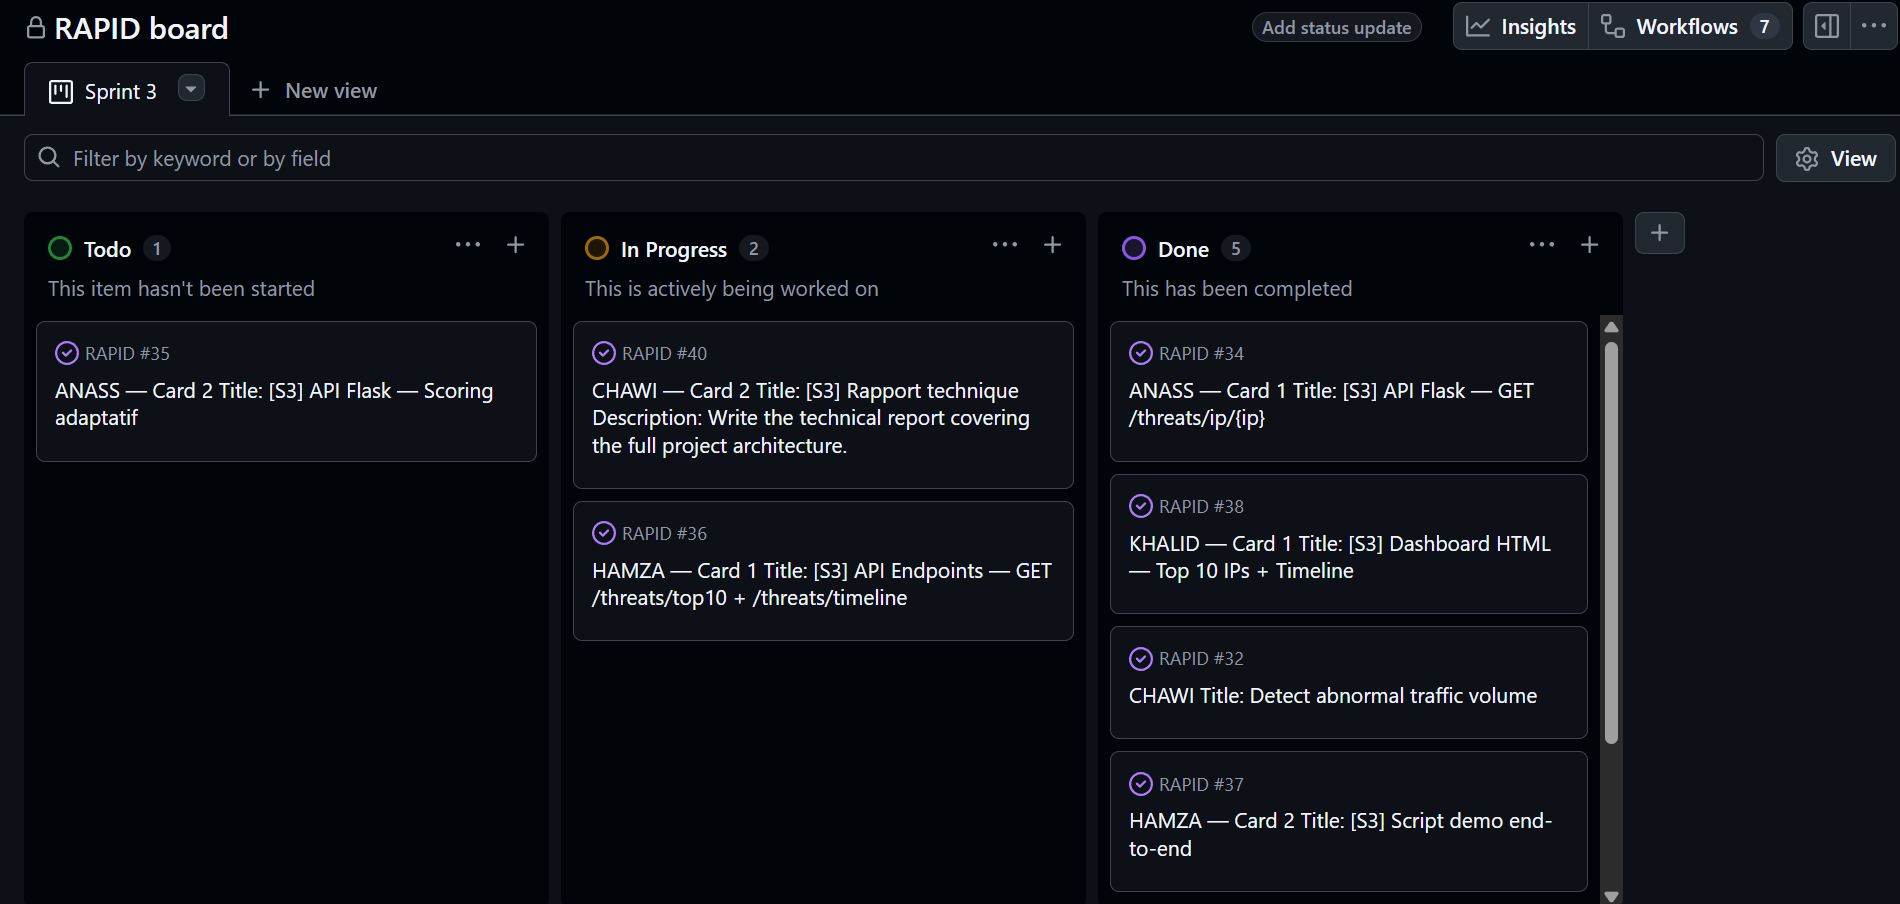
\includegraphics[width=\textwidth]{figures/board3.png}
    \caption{GitHub project board for Sprint 3, focused on API integration, dashboard delivery, demonstration, and reporting.}
    \label{fig:scrum-board-sprint3}
\end{figure}

\section{Tailscale and Docker Swarm Infrastructure}

The deployment uses two complementary networking mechanisms. Tailscale provides the private network between physical machines. Docker Swarm provides the container-level overlay network. These two layers solve different problems and are both necessary.

\subsection{Why Tailscale Is Used}

Tailscale gives each team machine a stable private address in the \texttt{100.x.x.x} range. This is important because the team is not working inside a single university data center with fixed servers. The machines may be on different local networks, behind NAT, or connected from different places. Without Tailscale, the team would have to expose ports publicly, configure router forwarding, or constantly change IP addresses in scripts and containers. That would make the deployment fragile and less secure.

With Tailscale, Kafka can be advertised as \texttt{100.73.216.115:9092}, Cassandra can be reached at \texttt{100.97.208.110:9042}, HBase Thrift can be reached at \texttt{100.97.208.110:9090}, and the Flask API can expose \texttt{100.73.216.115:5000}. This makes the distributed infrastructure predictable. It also keeps communication private because the services are intended to be accessed through the Tailscale mesh rather than through public Internet addresses \cite{tailscale_docs}.

\subsection{Why Docker Swarm Is Used}

Docker Compose alone is comfortable for a single host, but RAPID is intentionally multi-host. Docker Swarm adds the cluster concept needed to connect containers across machines \cite{docker_swarm_docs}. The external attachable network \texttt{rapid-overlay} allows containers started by different Compose profiles to communicate through one logical overlay. This means that a Spark container on one machine can reach Kafka on Anass' node and Cassandra on Chawi's node without pretending that all services are local.

The Compose profiles also enforce ownership. Anass starts only the \texttt{anass} profile, Hamza starts \texttt{hamza}, Khalid starts \texttt{khalid}, and Chawi starts \texttt{chawi}. This is cleaner than asking every team member to run the full infrastructure. It also mirrors real deployments where different teams or nodes own different services.

\begin{figure}[H]
    \centering
    \resizebox{\textwidth}{!}{\begin{tikzpicture}[
    font=\small,
    layer/.style={draw, rounded corners=6pt, minimum width=19.0cm, minimum height=2.35cm, fill=white},
    layername/.style={font=\bfseries, align=center},
    host/.style={draw, rounded corners=4pt, align=center, text width=3.35cm, minimum height=0.95cm, fill=white},
    service/.style={draw, rounded corners=4pt, align=center, text width=3.25cm, minimum height=1.08cm, fill=white},
    overlay/.style={draw, rounded corners=4pt, align=center, text width=15.4cm, minimum height=0.92cm, fill=rapidBlue!10},
    mesh/.style={thick, rapidGreen}
]

\node[layer, fill=rapidGreen!8] at (0,3.85) {};
\node[layername] at (0,4.65) {Layer 1: Tailscale host mesh};
\node[host, fill=rapidLight] (anassIp) at (-7.05,3.55) {Anass\\100.73.216.115};
\node[host, fill=rapidLight] (hamzaIp) at (-2.35,3.55) {Hamza\\100.72.34.26};
\node[host, fill=rapidLight] (khalidIp) at (2.35,3.55) {Khalid\\100.127.99.23};
\node[host, fill=rapidLight] (chawiIp) at (7.05,3.55) {Chawi\\100.97.208.110};

\draw[mesh] (anassIp.east) -- (hamzaIp.west);
\draw[mesh] (hamzaIp.east) -- (khalidIp.west);
\draw[mesh] (khalidIp.east) -- (chawiIp.west);

\node[layer, fill=rapidBlue!8] at (0,0.55) {};
\node[layername] at (0,1.35) {Layer 2: Docker Swarm overlay};
\node[overlay] (rapidOverlay) at (0,0.25) {\texttt{rapid-overlay}: shared container network across the four machines};

\node[layer, fill=rapidOrange!8] at (0,-2.85) {};
\node[layername] at (0,-2.05) {Layer 3: RAPID containers};
\node[service, fill=rapidGreen!12] (anassSvc) at (-7.05,-3.15) {Kafka\\HDFS\\Flask API};
\node[service, fill=rapidBlue!10] (hamzaSvc) at (-2.35,-3.15) {Spark master\\Spark worker};
\node[service, fill=rapidBlue!10] (khalidSvc) at (2.35,-3.15) {Spark streaming\\detectors};
\node[service, fill=rapidOrange!12] (chawiSvc) at (7.05,-3.15) {Cassandra\\HBase\\Dashboard};

\end{tikzpicture}
}
    \caption{Infrastructure layers: Tailscale connects the physical machines, while Docker Swarm provides the shared container overlay network.}
    \label{fig:tailscale-swarm-layers}
\end{figure}

\subsection{Operational Verification from Docker Screenshots}

The Docker Swarm deployment was verified from the command line by checking both node membership and running containers. Figure~\ref{fig:docker-node-status} shows that the machines were registered in the Swarm membership list. In that capture, some worker nodes appear as \texttt{Down}; this does not invalidate the deployment model, because student laptops can be temporarily offline, suspended, or disconnected from Tailscale when the manager runs \texttt{docker node ls}. For that reason, the stronger operational evidence is the per-machine \texttt{docker ps} output in Figures~\ref{fig:docker-ps-anass}--\ref{fig:docker-ps-chawi}, which shows the actual containers running on each owner machine.

\begin{figure}[H]
    \centering
    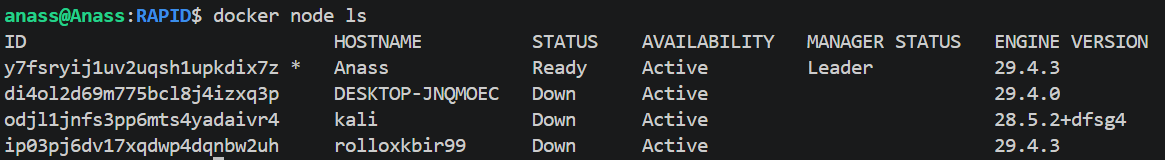
\includegraphics[width=\textwidth]{figures/dockernode.png}
    \caption{Docker Swarm node list on the manager machine. The list verifies node registration; temporary \texttt{Down} states reflect machine availability at screenshot time.}
    \label{fig:docker-node-status}
\end{figure}

\begin{figure}[H]
    \centering
    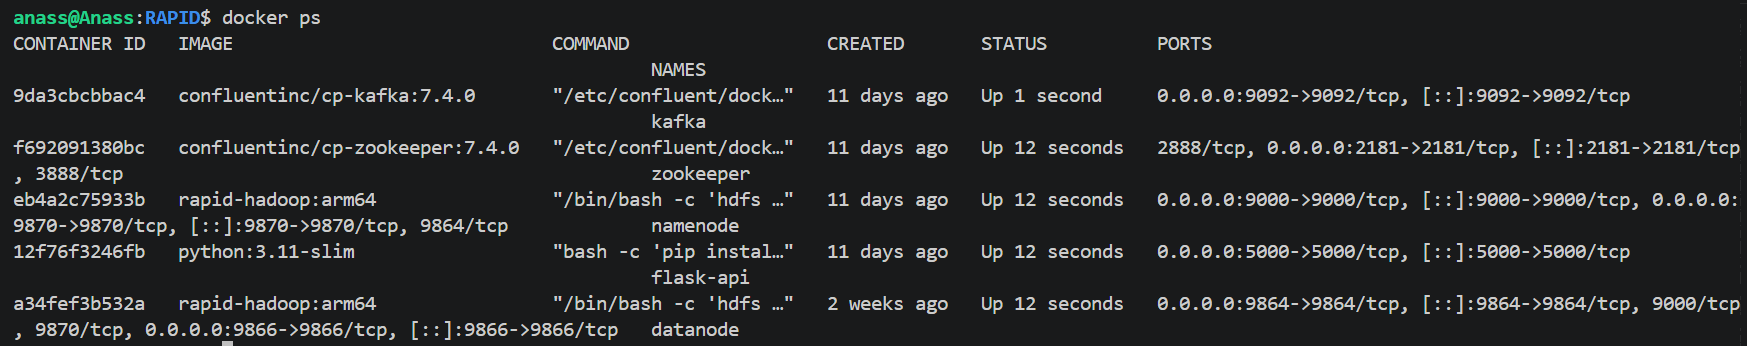
\includegraphics[width=\textwidth]{figures/dockerps1.png}
    \caption{Docker container status on Anass' machine, showing Kafka, Zookeeper, HDFS NameNode/DataNode, and the Flask API profile.}
    \label{fig:docker-ps-anass}
\end{figure}

\begin{figure}[H]
    \centering
    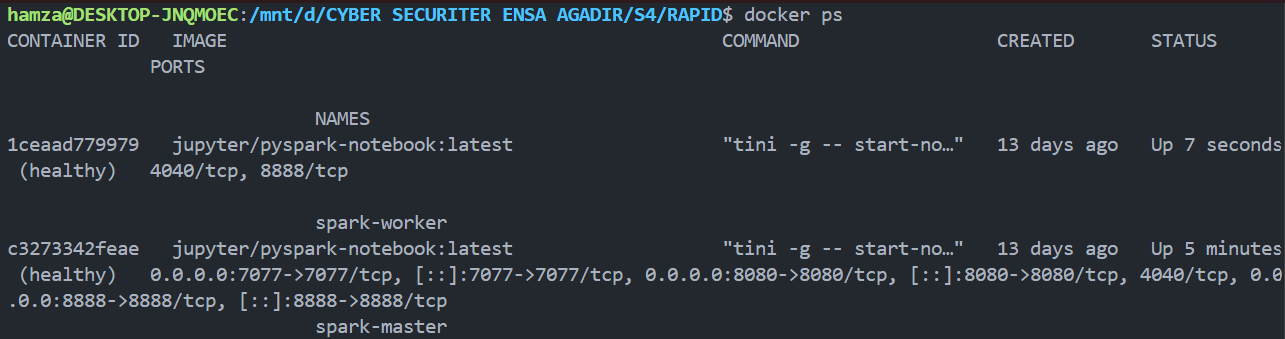
\includegraphics[width=\textwidth]{figures/docker_ps_hamza.png}
    \caption{Docker container status on Hamza's machine, showing the Spark master and Spark worker used for batch processing and Kafka replay work.}
    \label{fig:docker-ps-hamza}
\end{figure}

\begin{figure}[H]
    \centering
    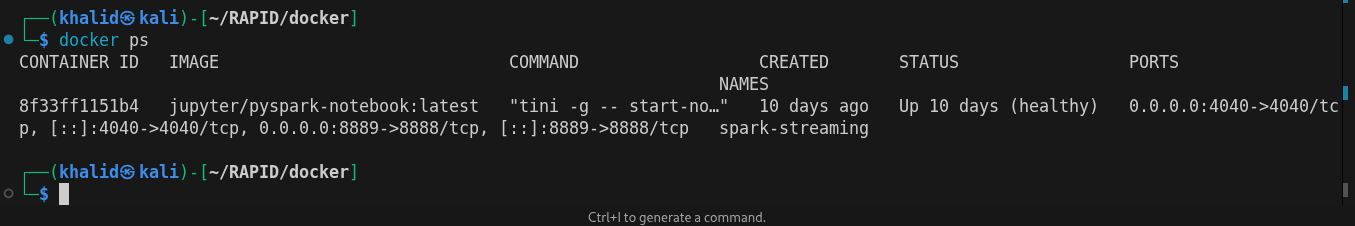
\includegraphics[width=\textwidth]{figures/docker_ps.png}
    \caption{Docker container status on Khalid's machine, showing the single Spark streaming container used for real-time detection jobs.}
    \label{fig:docker-ps-khalid}
\end{figure}

\begin{figure}[H]
    \centering
    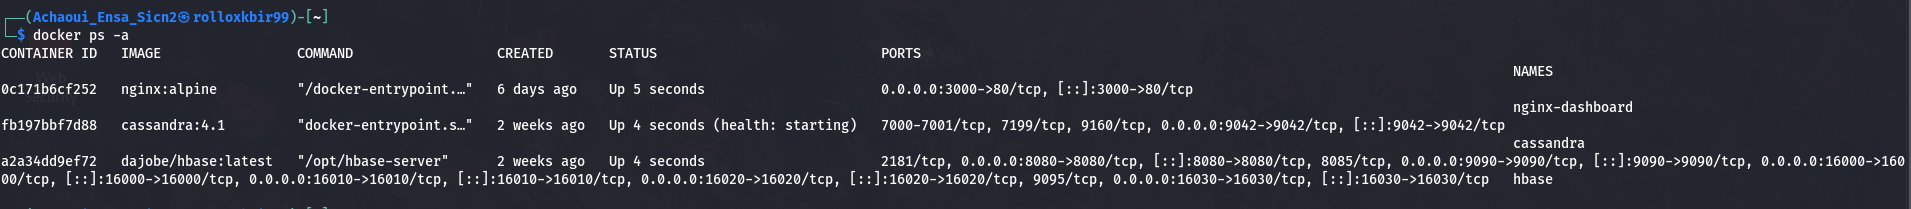
\includegraphics[width=\textwidth]{figures/docker_ps_chawi.png}
    \caption{Docker container status on Chawi's machine, showing Cassandra, HBase, and the Nginx dashboard container for the serving and visualization layer.}
    \label{fig:docker-ps-chawi}
\end{figure}

Together, these screenshots support the architectural claim made in the backlog: every member does not need to run the full stack. Anass carries the infrastructure gateway services, Hamza carries Spark batch execution, Khalid carries the lightweight streaming runtime, and Chawi carries the serving databases and dashboard host. The distribution is especially important for machines with lower memory capacity, because Cassandra, HBase, and Spark should not all be forced onto the same laptop during the demonstration.

\subsection{Runtime Communication}

Figure~\ref{fig:runtime-communication} shows how the services communicate during execution. The important point is that no component is isolated: Spark batch jobs read from HDFS and write HBase views, streaming jobs consume Kafka and write Cassandra views, and the Flask API reads both databases to serve the dashboard. The architecture therefore behaves like a small production cluster rather than a monolithic local script.

\begin{figure}[H]
    \centering
    \resizebox{\textwidth}{!}{\begin{tikzpicture}[
    font=\small,
    lane/.style={draw, rounded corners=6pt, minimum width=19.0cm, minimum height=1.9cm, fill=white},
    lanetitle/.style={font=\bfseries, align=left},
    svc/.style={draw, rounded corners=4pt, align=center, text width=4.0cm, minimum height=1.0cm, fill=white},
    arrow/.style={-{Latex[length=2.4mm]}, thick, shorten >=4pt, shorten <=4pt},
    stream/.style={arrow, rapidOrange},
    batch/.style={arrow, rapidBlue},
    query/.style={arrow, rapidGreen}
]

% Streaming lane.
\node[lane, fill=rapidOrange!8] at (0,2.35) {};
\node[lanetitle, text=rapidOrange] at (-7.0,3.05) {Streaming path};
\node[svc, fill=rapidOrange!12] (kafka) at (-6.3,2.18) {Anass\\Kafka broker};
\node[svc, fill=rapidOrange!12] (streaming) at (0,2.18) {Khalid\\Spark streaming jobs};
\node[svc, fill=rapidOrange!12] (cassWrite) at (6.3,2.18) {Chawi\\Cassandra views};
\draw[stream] (kafka.east) -- (streaming.west);
\draw[stream] (streaming.east) -- (cassWrite.west);

% Batch lane.
\node[lane, fill=rapidBlue!8] at (0,0) {};
\node[lanetitle, text=rapidBlue] at (-7.0,0.70) {Batch path};
\node[svc, fill=rapidBlue!10] (hdfs) at (-6.3,-0.17) {Anass\\HDFS raw logs};
\node[svc, fill=rapidBlue!10] (batchJobs) at (0,-0.17) {Hamza\\Spark batch jobs};
\node[svc, fill=rapidBlue!10] (hbase) at (6.3,-0.17) {Chawi\\HBase views};
\draw[batch] (hdfs.east) -- (batchJobs.west);
\draw[batch] (batchJobs.east) -- (hbase.west);

% Query lane.
\node[lane, fill=rapidGreen!8] at (0,-2.35) {};
\node[lanetitle, text=rapidGreen] at (-7.0,-1.65) {API path};
\node[svc, fill=rapidGreen!12] (stores) at (-6.3,-2.52) {Cassandra and HBase\\serving reads};
\node[svc, fill=rapidGreen!12] (api) at (0,-2.52) {Anass\\Flask API};
\node[svc, fill=rapidGreen!12] (dashboard) at (6.3,-2.52) {Chawi\\Dashboard};
\draw[query] (stores.east) -- (api.west);
\draw[query] (api.east) -- (dashboard.west);

\end{tikzpicture}
}
    \caption{Runtime communication between owner nodes. The arrows represent the main data and query paths used by the RAPID pipeline.}
    \label{fig:runtime-communication}
\end{figure}

\subsection{Physical Deployment}

The physical deployment uses stable private IP addresses instead of assuming that all services run on the same host. Table~\ref{tab:deployment-ownership} summarizes the ownership model. The Anass profile is the entry point of the data backbone because Kafka, HDFS, and the API are the services that connect the other layers together.

\begin{table}[H]
    \centering
    \caption{Distributed service ownership in the RAPID deployment.}
    \label{tab:deployment-ownership}
    \begin{tabularx}{\textwidth}{>{\bfseries}l l X}
        \toprule
        Owner & Tailscale address & Main services \\
        \midrule
        Anass & \texttt{100.73.216.115} & Zookeeper, Kafka broker, HDFS NameNode, HDFS DataNode, Flask REST API \\
        Hamza & \texttt{100.72.34.26} & Spark master, Spark worker, Jupyter/Spark development environment \\
        Khalid & \texttt{100.127.99.23} & Spark streaming container and real-time detection jobs \\
        Chawi & \texttt{100.97.208.110} & Cassandra, HBase Thrift service, HBase UI, dashboard hosting \\
        \bottomrule
    \end{tabularx}
\end{table}

This deployment model provides a practical simulation of real-life big-data infrastructure. A production platform normally does not place brokers, distributed storage, compute engines, serving databases, and APIs on one machine. RAPID follows the same principle at project scale. The platform separates concerns, keeps the raw data and derived views rebuildable, and gives every service a clear network endpoint.

\section{Rationale for a Lambda Architecture}

A cybersecurity monitoring system must answer two different classes of questions. Some questions are historical: which IP addresses were repeatedly malicious during the month, which protocols were most affected, and which attack patterns were observed across the dataset? Other questions are operational: did a source IP just trigger a brute-force pattern, is the current volume abnormal, and should the dashboard recommend blocking or monitoring an IP? A single processing model is poorly suited to both workloads. Batch processing provides accuracy and completeness, but it is not optimized for immediate alerts. Pure streaming provides freshness, but it is less convenient for recomputing large historical views when logic changes or when late data is found.

The Lambda Architecture separates these concerns into a batch layer, a speed layer, and a serving layer \cite{marz2011lambda,marz2015bigdata}. RAPID applies this idea as follows:

\begin{itemize}
    \item The \textbf{batch layer} reads the complete log corpus from HDFS and computes historical indicators such as IP reputation, attack patterns, threat timelines, port-scan summaries, and volume-by-threat statistics.
    \item The \textbf{speed layer} consumes events from Kafka and updates Cassandra with recent logs, signature alerts, volume alerts, brute-force detections, and threat scores.
    \item The \textbf{serving layer} exposes both views through Flask. The API does not force the client to know whether an answer is historical or real-time; it joins the relevant evidence and returns a decision-ready JSON document.
\end{itemize}

This design also supports replay. Since the producer reads HDFS partitions and publishes events to Kafka, the team can replay the dataset into the speed layer after changing a streaming rule. Reproducibility is essential in an academic project because the same dataset can be used to verify each processing stage under controlled conditions.

\section{Technology Choices}

\subsection{Kafka for Ingestion and Decoupling}

Kafka was selected as the ingestion backbone because it is designed for durable, ordered event streams and for decoupling producers from consumers \cite{kafka_docs}. In RAPID, the topic \texttt{cybersecurity-logs} receives JSON events generated from HDFS monthly partitions. The Kafka producer uses \texttt{source\_ip} as the message key, which keeps related events naturally grouped for downstream processing. The producer also maintains a small state file so that an interrupted replay can resume from the last month and line number instead of restarting the full dataset.

The main architectural benefit of Kafka is that it protects the streaming jobs from direct dependency on HDFS reads. Spark streaming jobs consume from Kafka at their own pace, and additional detection jobs can be attached to the same topic without changing the producer. For security analytics, this matters because new detectors are often added iteratively: a brute-force detector, a signature detector, a volume detector, and a score aggregator can all observe the same event stream while writing separate serving tables.

\subsection{HDFS for the Raw, Replayable Dataset}

HDFS is used as the durable storage layer for the raw cybersecurity logs. The current convention stores monthly partitions under paths such as \texttt{/logs/year=2024/month=01/data.csv}. HDFS is appropriate here because it is built for large files, sequential reads, and distributed storage \cite{hdfs_docs}. The partition layout makes it possible to process the complete dataset for batch analytics and to replay selected months through Kafka when validating the speed layer.

The role of HDFS is not only storage capacity. It is also the audit base of the architecture. If a derived table in Cassandra or HBase becomes inconsistent, the raw partitioned data remains available for recomputation. This property is a core reason why Lambda Architecture is useful in analytical systems: derived views can be rebuilt from immutable input data when algorithms evolve.

\subsection{Spark for Unified Batch and Streaming Computation}

Spark was selected because it provides a single programming environment for batch processing and streaming analytics \cite{spark_docs}. The batch jobs in \texttt{spark/batch/} compute historical views such as malicious IP rankings, port scans, attack paths, HBase threat timelines, multi-step attacks, and volume statistics. The streaming jobs in \texttt{spark/streaming/} consume Kafka using Structured Streaming and write results to Cassandra \cite{spark_streaming_docs}.

Using Spark in both layers reduces conceptual fragmentation. The same schema fields, such as \texttt{timestamp}, \texttt{source\_ip}, \texttt{dest\_ip}, \texttt{protocol}, \texttt{action}, \texttt{threat\_label}, \texttt{bytes\_transferred}, \texttt{user\_agent}, and \texttt{request\_path}, are transformed across the batch and speed jobs. This makes the results easier to compare and makes future maintenance simpler.

\subsection{Cassandra for Real-Time Serving Views}

Cassandra was selected for the speed layer serving store because it is a distributed wide-column database optimized for high-write workloads and predictable key-based reads \cite{cassandra_docs}. RAPID's streaming jobs write frequently updated operational views into the \texttt{cybersecurity} keyspace. The Flask API reads from tables such as \texttt{logs}, \texttt{realtime\_threats}, \texttt{signature\_alerts}, \texttt{volume\_alerts}, and \texttt{threat\_scores}.

The data model follows the access patterns of the API. For example, \texttt{/threats/ip/<ip>} reads the latest real-time threat state, score, signature alerts, and volume alerts for a source IP. \texttt{/threats/top10} scans the scoring table and sorts the highest-risk sources for dashboard presentation. The design favors fast operational lookup over ad-hoc relational joins, which is consistent with Cassandra's strengths.

\subsection{HBase for Historical Reputation and Time-Series Views}

HBase was selected for historical and batch-generated views because it provides sparse, versioned, column-family-oriented storage on top of the Hadoop ecosystem \cite{hbase_docs}. In RAPID, HBase stores tables such as \texttt{ip\_reputation}, \texttt{attack\_patterns}, and \texttt{threat\_timeline}. These tables are produced by batch jobs and accessed through the HBase Thrift service from the Flask API.

HBase complements Cassandra rather than replacing it. Cassandra serves recent state generated by the streaming layer, while HBase stores historical evidence computed from the complete dataset. For instance, the API uses HBase \texttt{ip\_reputation} values such as threat counts, SQL injection hits, tool hits, traversal hits, cross-site scripting hits, and average transferred bytes to calculate a normalized historical score. This historical score is then compared with current Cassandra scores to produce a final decision.

\section{Data Flow and Processing Contracts}

The architecture relies on explicit contracts between stages. The ingestion schema contains the timestamp, source and destination IP addresses, protocol, action, threat label, log type, transferred bytes, user agent, and request path. These fields are carried as JSON through Kafka and converted by Spark into typed columns. The base streaming writer persists the raw stream into Cassandra \texttt{logs}; specialized jobs then derive detector-specific tables.

\begin{longtable}{
    >{\raggedright\arraybackslash\bfseries}p{0.23\textwidth}
    >{\raggedright\arraybackslash}p{0.29\textwidth}
    >{\raggedright\arraybackslash}p{0.36\textwidth}
}
    \caption{Main data contracts between RAPID components.}
    \label{tab:data-contracts}\\
    \toprule
    Contract & Producer & Consumer or destination \\
    \midrule
    \endfirsthead
    \toprule
    Contract & Producer & Consumer or destination \\
    \midrule
    \endhead
    HDFS raw partitions & Dataset loader and storage preparation scripts & Kafka replay producer and Spark batch jobs \\
    Kafka JSON events & \texttt{spark/speed\_layer/}\newline\texttt{kafka\_producer.py} & Spark streaming writer and detection jobs \\
    Cassandra raw logs & Base streaming writer & API timeline, protocol aggregation, adaptive threshold, geo endpoint \\
    Cassandra alert views & Signature, brute-force, volume, and score streaming jobs & API threat lookup, recent alerts, top 10, volume endpoint \\
    HBase historical views & Spark batch jobs & API historical reputation and long-term trend lookup \\
    REST JSON responses & Flask API & Dashboard, smoke tests, integration tests, and external clients \\
    \bottomrule
\end{longtable}

This contract-based design reduces coupling. For example, a new streaming detector can write a new Cassandra view without changing the raw HDFS layout. Similarly, a batch job can improve the HBase reputation formula while the REST endpoint continues to return the same high-level fields to the dashboard.

\section{Flask API as the Serving Bridge}

The Flask API is the integration point between storage systems and client applications \cite{flask_docs}. It runs on Anass' node and connects to Cassandra and HBase through environment-configured hosts. Its purpose is not merely to expose database rows; it transforms distributed evidence into a security decision. Figure~\ref{fig:api-bridge} shows this bridge.

\begin{figure}[H]
    \centering
    \resizebox{\textwidth}{!}{\begin{tikzpicture}[
    font=\small,
    box/.style={draw, rounded corners=3pt, align=center, minimum height=0.95cm, text width=3.35cm, fill=white},
    db/.style={draw, cylinder, shape border rotate=90, aspect=0.23, align=center, minimum height=1.1cm, text width=3.05cm, fill=white},
    arrow/.style={-{Latex[length=2.3mm]}, thick, shorten >=2pt, shorten <=2pt},
    query/.style={arrow, rapidBlue},
    result/.style={arrow, rapidGreen}
]

\node[box, fill=rapidLight] (client) at (0,0) {Dashboard, tests,\\or analyst client};
\node[box, fill=rapidGreen!12] (flask) at (4.9,0) {Flask API\\\texttt{app.py}};

\node[db, fill=rapidOrange!12] (cass) at (9.5,2.0) {Cassandra\\\texttt{logs}\\\texttt{threat\_scores}\\\texttt{realtime\_threats}\\\texttt{signature\_alerts}\\\texttt{volume\_alerts}};
\node[db, fill=rapidBlue!10] (hbase) at (9.5,-2.0) {HBase\\\texttt{ip\_reputation}\\\texttt{attack\_patterns}\\\texttt{threat\_timeline}};

\node[box, fill=rapidLight] (rt) at (13.8,2.0) {Recent state\\alerts, scores, windows};
\node[box, fill=rapidLight] (hist) at (13.8,-2.0) {Historical context\\reputation and trends};
\node[box, fill=rapidGreen!12] (decision) at (18.2,0) {Merged JSON\\score, level,\\recommendation};

\draw[query] (client) -- (flask);
\node[fill=white, inner sep=1.5pt, text=rapidBlue] at (2.45,0.47) {HTTP GET};
\draw[query] (flask.east) -- ++(0.45,0) |- (cass.west);
\draw[query] (flask.east) -- ++(0.45,0) |- (hbase.west);

\draw[result] (cass) -- (rt);
\draw[result] (hbase) -- (hist);
\draw[result] (rt.east) -- ++(0.55,0) |- (decision.north);
\draw[result] (hist.east) -- ++(0.55,0) |- (decision.south);
\draw[result] (decision.south) |- ++(0,-3.25) -| node[pos=0.88, below, fill=white, inner sep=1.5pt]{JSON response} (client.south);

\end{tikzpicture}
}
    \caption{Flask API bridge: operational Cassandra views and historical HBase views are merged into decision-ready JSON responses.}
    \label{fig:api-bridge}
\end{figure}

\subsection{Connection Strategy}

The API keeps a persistent Cassandra session with a lightweight health query before reuse. If the session fails, it shuts down the old cluster handle and reconnects. This is useful in a distributed student deployment where containers may restart independently. HBase access is performed through HappyBase over the Thrift port \texttt{9090}. The environment variables \texttt{CASSANDRA\_HOST}, \texttt{HBASE\_HOST}, and \texttt{HDFS\_HOST} allow the same API code to run even if the physical node addresses change.

\subsection{Endpoint Responsibilities}

Table~\ref{tab:api-endpoints} summarizes the endpoints implemented in \texttt{bigdata-api/app.py}. The most important endpoint is \texttt{/threats/ip/<ip>} because it demonstrates the bridge between databases. It queries Cassandra for real-time state and HBase for historical reputation, computes a final score, compares it with the adaptive threshold, and returns a recommendation.

\begin{longtable}{>{\ttfamily}p{0.29\textwidth} p{0.27\textwidth} p{0.34\textwidth}}
    \caption{Flask API endpoints and their role in the serving layer.}
    \label{tab:api-endpoints}\\
    \toprule
    Endpoint & Main data source & Returned information \\
    \midrule
    \endfirsthead
    \toprule
    Endpoint & Main data source & Returned information \\
    \midrule
    \endhead
    GET /health & Runtime configuration & API status, backend hosts, HBase port, Cassandra keyspace \\
    GET /threats/ip/<ip> & Cassandra and HBase & Real-time threats, threat score, signatures, volume alerts, historical reputation, final score, threat level, recommendation \\
    GET /threats/top10 & Cassandra \texttt{threat\_scores} & Highest scored source IPs with malicious, suspicious, and total event counts \\
    GET /threats/threshold & Cassandra \texttt{logs} & Rolling 24-hour adaptive threshold and calculation metadata \\
    GET /threats/recent & Cassandra \texttt{signature\_alerts} & Most recent signature-based alerts \\
    GET /threats/volume-alerts & Cassandra \texttt{volume\_alerts} & Recent traffic-volume anomalies and detection windows \\
    GET /threats/by-protocol & Cassandra \texttt{logs} & Total, malicious, and suspicious counts grouped by protocol \\
    GET /threats/timeline & Cassandra \texttt{logs} & Daily threat counts used by timeline visualizations \\
    GET /threats/geo/attacks & Cassandra \texttt{logs} and \texttt{threat\_scores} & Public-IP attack arcs with inferred type, severity, geolocation, and score metadata \\
    \bottomrule
\end{longtable}

\subsection{Threat Score Fusion}

The \texttt{/threats/ip/<ip>} endpoint follows a clear fusion process. First, it retrieves real-time rows from Cassandra: active threat state, aggregated score, signature alerts, and volume alerts. Second, it retrieves historical HBase reputation for the same IP. Third, it converts the HBase values into a normalized score between 0 and 100. The historical formula gives weight to repeated threat counts, SQL injection indicators, scanner/tool indicators, path traversal, cross-site scripting, and average bytes transferred. Fourth, the endpoint takes the maximum of available real-time and historical scores as the final score.

This maximum-score strategy is intentionally conservative. In security monitoring, an IP should not be considered safe only because one evidence source is quiet. A source can be historically dangerous even if it has no recent alert, or it can be currently dangerous even without long historical presence. Combining the strongest available evidence makes the recommendation more cautious and therefore more appropriate for threat triage.

\subsection{Adaptive Thresholding}

The API includes an adaptive threshold calculation over a rolling 24-hour window. It scans recent Cassandra log rows, converts each event into a normalized score, computes the average score in the window, and sets the threshold using:

\[
    threshold = \min(avg\_score\_{24h} \times 1.5, 100)
\]

The score function incorporates the threat label, blocked actions, known offensive tool indicators such as SQLMap or Nmap, path traversal markers, brute-force indicators, XSS markers, and transferred bytes. The endpoint returns both the threshold and metadata such as sample count, reference time, window start, multiplier, and formula. This makes the decision process auditable instead of returning a hidden constant.

\subsection{Recommendation Policy}

The API maps the final score to an operational recommendation using the adaptive threshold. If the final score is above the threshold, the IP is classified as \texttt{HIGH} and the recommendation is \texttt{BLOCK}. If it is at least 70\% of the threshold, it is classified as \texttt{MEDIUM} and the recommendation is \texttt{MONITOR}. Otherwise, it is classified as \texttt{LOW} and the recommendation is \texttt{ALLOW}. This policy is simple enough to explain in a report and practical enough for a dashboard.

\section{Reliability, Reproducibility, and Security Considerations}

Several implementation choices improve the reliability of the backbone:

\begin{itemize}
    \item The Kafka producer persists replay progress in \texttt{/tmp/kafka\_producer\_state.json}, which prevents complete restart after interruption.
    \item Spark streaming jobs use checkpoint locations so that streaming progress can be recovered between runs.
    \item The API reconnects to Cassandra when a session becomes invalid.
    \item HDFS keeps raw data separate from derived views, making Cassandra and HBase tables rebuildable.
    \item Docker Compose profiles keep service ownership explicit and reduce the risk of starting conflicting containers on the wrong node.
\end{itemize}

Security is also considered at the architecture level. The services are intended to communicate over private Tailscale addresses and the Swarm overlay network rather than public interfaces. The API enables broad CORS for dashboard and demonstration convenience, but this should be restricted before production exposure. The geolocation endpoint only maps public source IPs and avoids treating private infrastructure IPs as real attack origins.

\section{Conclusion}

The backbone of RAPID combines Kafka, HDFS, Spark, Cassandra, HBase, and Flask into a coherent Lambda Architecture. Kafka gives the platform a replayable event stream, HDFS preserves the raw dataset, Spark implements both batch and speed computations, Cassandra serves recent operational state, HBase stores historical reputation, and Flask exposes a unified decision API. This architecture is appropriate for cybersecurity analytics because it balances freshness, historical accuracy, reproducibility, and client-facing simplicity.
